\documentclass{beamer}
\usetheme{Frankfurt}
% \setbeameroption{show notes}
% \setbeamertemplate{note page}[plain]

\usepackage[T1]{fontenc}
\usepackage[utf8]{inputenc}
\usepackage[french,english]{babel}

\usepackage{blindtext}
\usepackage{appendixnumberbeamer}

\title{Experiments on automation of formal verification of devices at the binary level}
\subtitle{}
\author{Thomas Lacroix}
\titlegraphic{
\includegraphics[width=4cm]{logos/insa-logo-coul.png}}
\institute{INSA Lyon \\ Soutenance de PFE (Option R\&D)}
\date{19/06/2019}

% Add pages before every section and subsections
\AtBeginSection[]{\frame{\sectionpage}}
\AtBeginSubsection[]
{%
    \begin{frame}
        \frametitle{Table of Contents}
        \tableofcontents[hideothersubsections, currentsection, currentsubsection]
    \end{frame}
}

% Add page number in upper-right corner
\makeatletter
\defbeamertemplate*{headline}{my smoothbars theme}
{%
    \pgfuseshading{beamer@barshade}%
    \ifbeamer@sb@subsection%
    \vskip-9.75ex%
    \else%
    \vskip-7ex%
    \fi%
    \begin{beamercolorbox}[ignorebg,ht=2.25ex,dp=3.75ex]{section in head/foot}
    \insertnavigation{.9\paperwidth}\hfill%
    \insertframenumber/\inserttotalframenumber%
    \hspace{.5em}
    \end{beamercolorbox}%
    \ifbeamer@sb@subsection%
    \begin{beamercolorbox}[ignorebg,ht=2.125ex,dp=1.125ex,%
        leftskip=.3cm,rightskip=.3cm plus1fil]{subsection in head/foot}
        \usebeamerfont{subsection in head/foot}\insertsubsectionhead
    \end{beamercolorbox}%
    \fi%
}%
\makeatother

% To remove the navigation buttons at the bottom
% \beamertemplatenavigationsymbolsempty

% Explain NIC and what we want to prove
%   - obvious reason: connected to Internet and DMA access
%   - buffer descriptor
%       - not circular
%       - only readable memory
%       - not overlapping
%   - show that it's possible to violate the invariant
%       -> overlapping tx and rx BD
%   => need to model the spec
%   => modeled with invariants
%
% Can we reuse work done for software verification to verify hardware?
%
% Start with explanation of PP analysis vs non-PP
%
% Last 5 minutes, show every supporting tools
%   => everything that is needed that is not direct PP stuff

%%%%%%%%%%%%%%%%%%%%%%%%%%%%%%%%%%%%%%%%%%%%%%%%%%%%%%%%%%%%%%%%%%%%%%%%%%%%%%%%
%%%%%%%%%%%%%%%%%%%%%%%%%%%%%%%%%%%%%%%%%%%%%%%%%%%%%%%%%%%%%%%%%%%%%%%%%%%%%%%%
%%%%%%%%%%%%%%%%%%%%%%%%%%%%%%%%%%%%%%%%%%%%%%%%%%%%%%%%%%%%%%%%%%%%%%%%%%%%%%%%

\begin{document}

\begin{frame}
    \maketitle
\end{frame}

%%%%%%%%%%%%%%%%%%%%%%%%%%%%%%%%%%%%%%%%%%%%%%%%%%%%%%%%%%%%%%%%%%%%%%%%%%%%%%%%
%%%%%%%%%%%%%%%%%%%%%%%%%%%%%%%%%%%%%%%%%%%%%%%%%%%%%%%%%%%%%%%%%%%%%%%%%%%%%%%%
%%%%%%%%%%%%%%%%%%%%%%%%%%%%%%%%%%%%%%%%%%%%%%%%%%%%%%%%%%%%%%%%%%%%%%%%%%%%%%%%

\section{Motivation}

\subsection{Formal verification}

\begin{frame}
    \note{
        Provers: generate a proof or not -> need tests or trustworthy
    }
\end{frame}

\begin{frame}{HOL4}
\end{frame}

\begin{frame}{Proof-producing analysis}
    \textit{Machine-checked proofs}
\end{frame}

\subsection{Security critical systems}

\begin{frame}{Security critical systems}
    \begin{columns}
        \begin{column}{0.5\textwidth}
            Privacy

            \begin{itemize}
                \item Smartphones
                \item Smart TVs
            \end{itemize}
        \end{column}
        \begin{column}{0.5\textwidth}
            Security

            \begin{itemize}
                \item Hospital equipment
                \item Traffic control systems
                \item Power plants
            \end{itemize}
        \end{column}
    \end{columns}
\end{frame}

\begin{frame}{Security critical systems - vulnerable}
    \begin{columns}
        \begin{column}{0.5\textwidth}
            https://www.wired.com/2014/04/ hospital-equipment-vulnerable/

            It's Insanely Easy to Hack Hospital Equipment
        \end{column}
        \begin{column}{0.5\textwidth}
            https://www.wired.com/2015/07/ hackers-remotely-kill-jeep-highway/

            Hackers Remotely Kill a Jeep on the Highway—With Me in It
        \end{column}
    \end{columns}
\end{frame}

\begin{frame}{Security critical systems - vulnerable}
    Vulnerabilities come because of:
    \begin{itemize}
        \item Increased surface of attack (more and more features, codebases explode in size)
        \item Connected to networks $\rightarrow$ remote attacks
    \end{itemize}

    \note{Often a result of misconfiguration.}
\end{frame}

\begin{frame}{Secure operating systems}
    \begin{columns}
        \begin{column}{0.4\textwidth}
            \begin{center}
                
\includegraphics[height=2cm]{logos/seL4-logo-text-white.png}
            \end{center}
        \end{column}
        \pause
        \begin{column}{0.6\textwidth}
            Formal proof\footnotemark:
            \begin{itemize}
                \item The binary code correctly implements its \textbf{abstract specification}.
                \item The specification guarantees \textbf{integrity} and \textbf{confidentiality}.
            \end{itemize}

            \bigskip
            \pause

            \begin{itemize}
                \item \textbf{Integrity}: data cannot be \textit{changed} without permission.
                \item \textbf{Confidentiality}: data cannot be \textit{read} without permission.
            \end{itemize}
        \end{column}
    \end{columns}
    \footnotetext{\tiny \url{https://sel4.systems/Info/FAQ/proof.pml}}
\end{frame}

\begin{frame}{Secure operating systems}
    \begin{columns}
        \begin{column}{0.4\textwidth}
            \begin{center}
                
\includegraphics[height=2cm]{logos/seL4-logo-text-white.png}
            \end{center}
        \end{column}
        \begin{column}{0.6\textwidth}
            Proof assumptions\footnotemark:
            \pause
            \begin{itemize}
                \item Use of Direct Memory Access (DMA) is excluded, or only allowed for \textbf{trusted drivers that have to be formally verified by the user}.
            \end{itemize}

            \note{Ongoing work: IOMMUs on x86 or System MMUs on ARM.}
        \end{column}
    \end{columns}
    \footnotetext{\tiny\url{https://docs.sel4.systems/FrequentlyAskedQuestions\#is-sel4-proven-secure}}
\end{frame}

\begin{frame}
    \begin{center}
        \begin{figure}
            \only<1|handout:0>{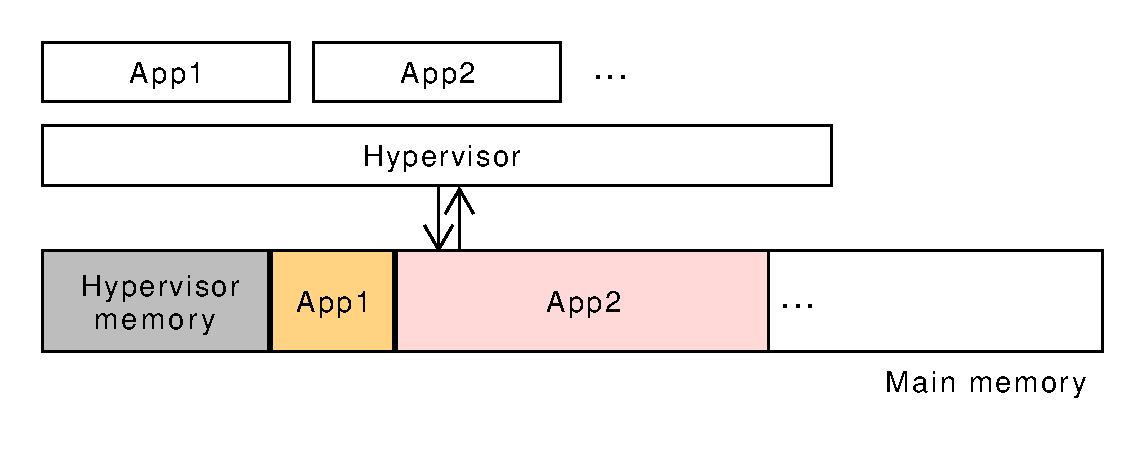
\includegraphics[width=\textwidth]{figures/dma-hyp-apps-nodma.pdf}}
            \only<2>{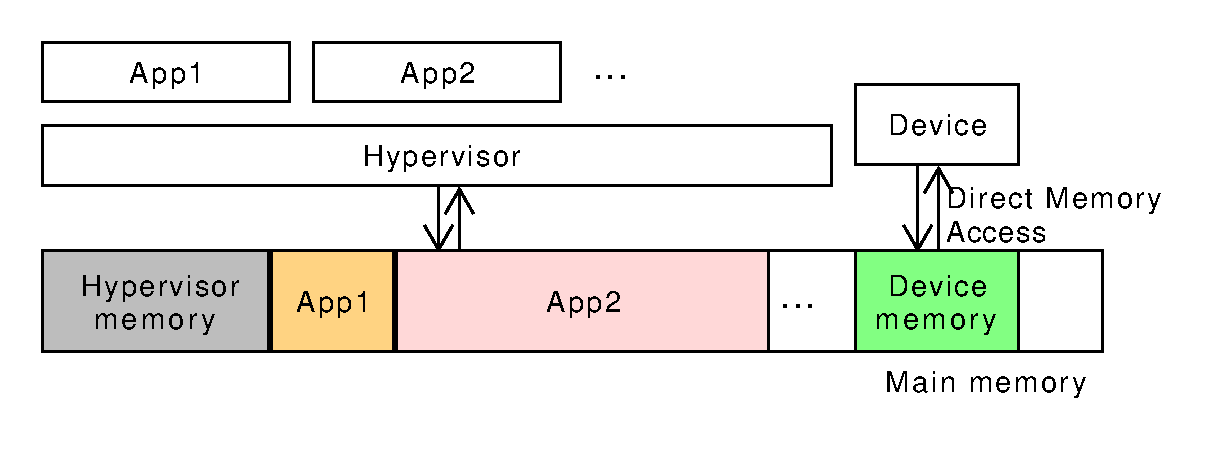
\includegraphics[width=\textwidth]{figures/dma-hyp-apps.pdf}}
            \label{dma-dangers-1}
        \end{figure}
    \end{center}
\end{frame}

\begin{frame}
    \begin{center}
        \begin{figure}
            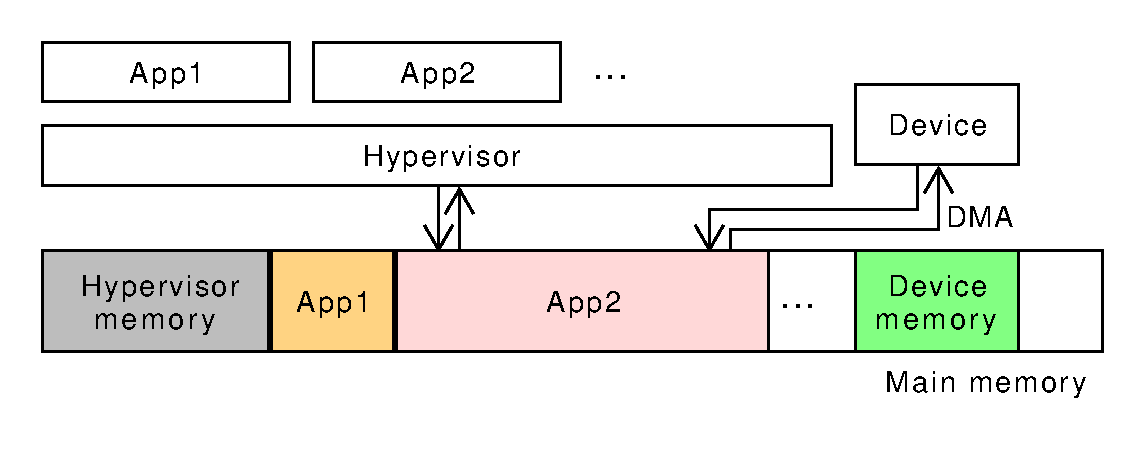
\includegraphics[width=\textwidth]{figures/dma-hyp-apps-bad.pdf}
            \label{dma-dangers-2}
        \end{figure}
    \end{center}
\end{frame}

\subsection{Network Interface Controllers (NIC)}

\begin{frame}
    \begin{figure}
        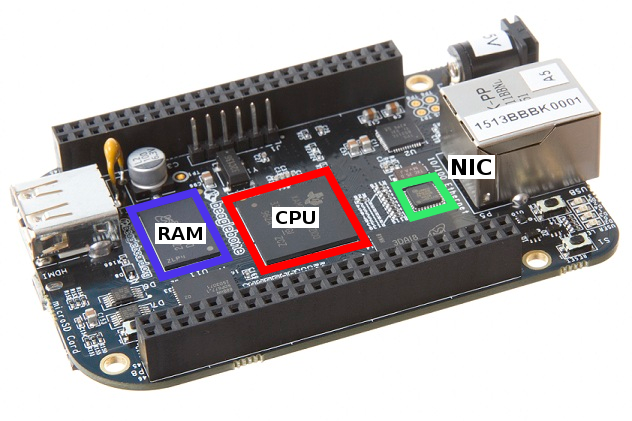
\includegraphics[]{figures/BBB_cpu_ram_nic.png}
        \caption{BeagleBone Black.}
        \label{bbb_nic}
    \end{figure}
\end{frame}

\begin{frame}
    \begin{figure}
        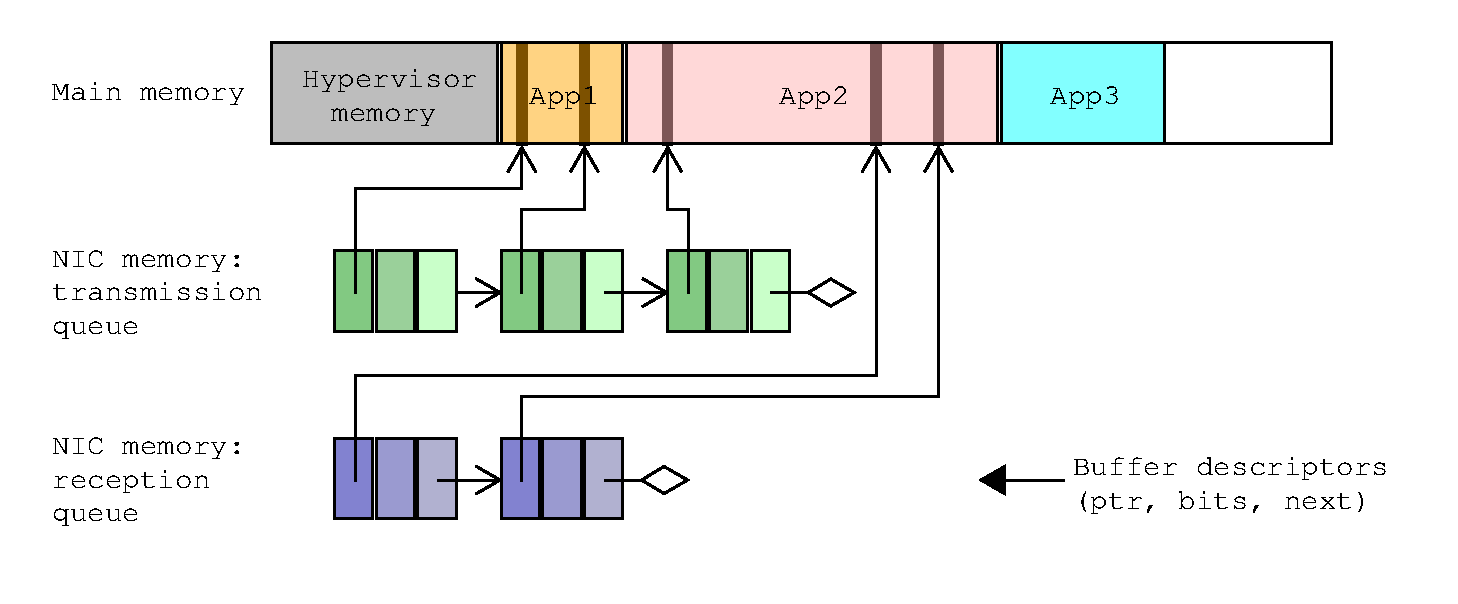
\includegraphics[width=\textwidth]{figures/nic-bd.pdf}
        \label{nic_bd}
    \end{figure}
\end{frame}

\begin{frame}
    \begin{figure}
        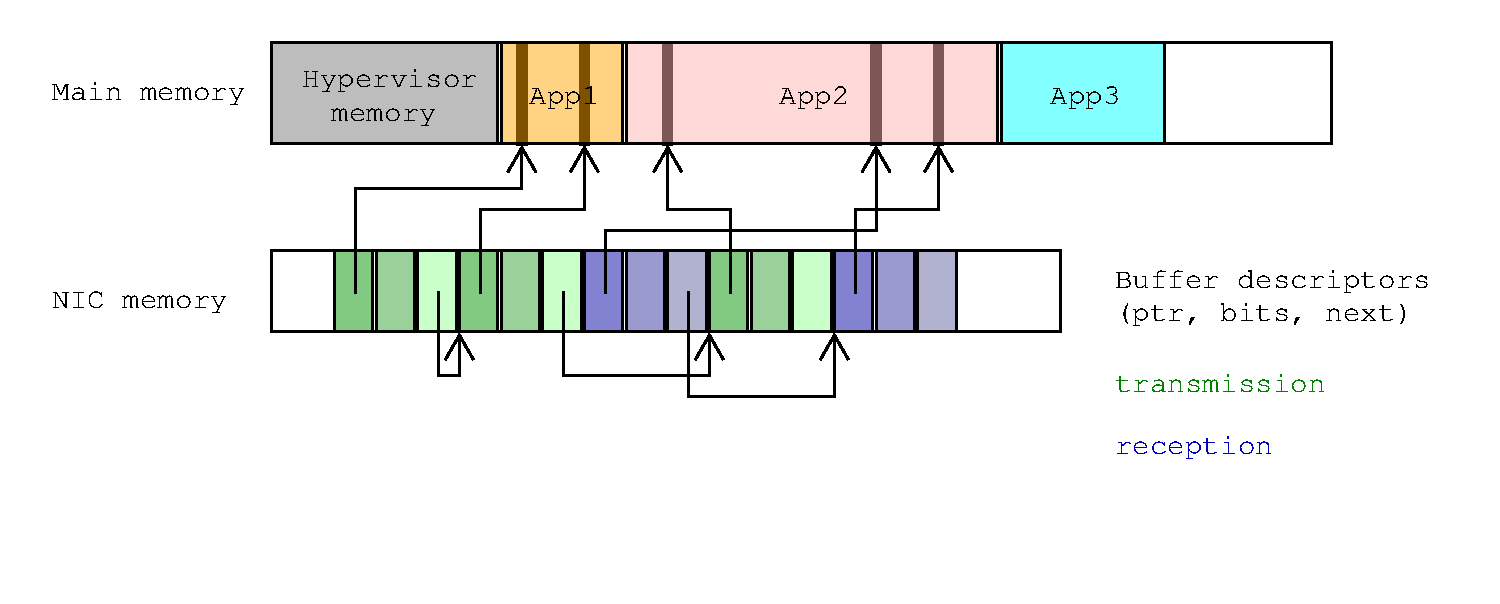
\includegraphics[width=\textwidth]{figures/nic-bd-in_mem.pdf}
        \label{nic_bd_inmem}
    \end{figure}
\end{frame}

\begin{frame}
    \begin{figure}
        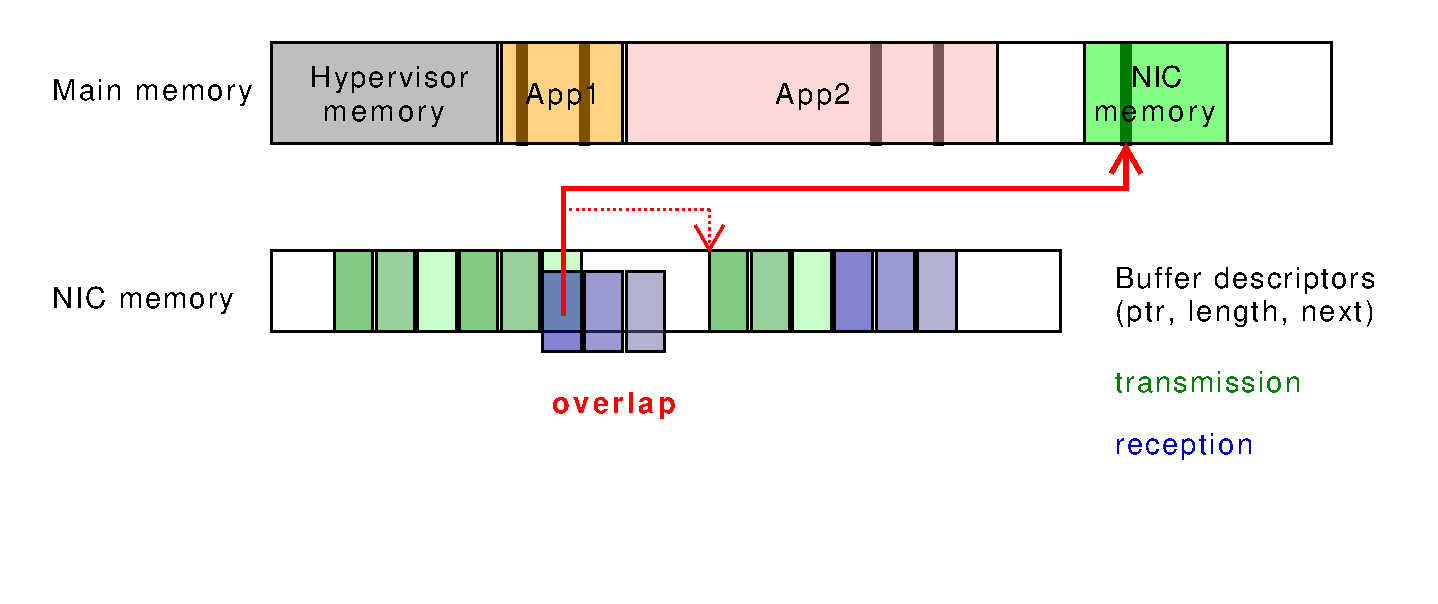
\includegraphics[width=\textwidth]{figures/nic-bd-in_mem-overlap.pdf}
        \label{nic_bd_inmem_overlap}
    \end{figure}
    \note{Figure 32 in Jonas' MT}
\end{frame}

\begin{frame}{Research question}
    \begin{center}
        \textbf{Can we apply traditional software verification techniques and tools to show security properties of hardware devices?}
    \end{center}
\end{frame}

%%%%%%%%%%%%%%%%%%%%%%%%%%%%%%%%%%%%%%%%%%%%%%%%%%%%%%%%%%%%%%%%%%%%%%%%%%%%%%%%
%%%%%%%%%%%%%%%%%%%%%%%%%%%%%%%%%%%%%%%%%%%%%%%%%%%%%%%%%%%%%%%%%%%%%%%%%%%%%%%%
%%%%%%%%%%%%%%%%%%%%%%%%%%%%%%%%%%%%%%%%%%%%%%%%%%%%%%%%%%%%%%%%%%%%%%%%%%%%%%%%

\section{Non proof-producing verification}

\subsection{Subsection 1}

\begin{frame}{Title}
\end{frame}

\subsection{How trustful is it?}

\begin{frame}{Title}
\end{frame}

\section{Proof-producing verification}

\subsection{Subsection 1}

\begin{frame}{Title}
\end{frame}

%%%%%%%%%%%%%%%%%%%%%%%%%%%%%%%%%%%%%%%%%%%%%%%%%%%%%%%%%%%%%%%%%%%%%%%%%%%%%%%%
%%%%%%%%%%%%%%%%%%%%%%%%%%%%%%%%%%%%%%%%%%%%%%%%%%%%%%%%%%%%%%%%%%%%%%%%%%%%%%%%
%%%%%%%%%%%%%%%%%%%%%%%%%%%%%%%%%%%%%%%%%%%%%%%%%%%%%%%%%%%%%%%%%%%%%%%%%%%%%%%%

\section{Conclusion}

\begin{frame}
    \begin{center}
        \huge
        Questions
    \end{center}
\end{frame}

%%%%%%%%%%%%%%%%%%%%%%%%%%%%%%%%%%%%%%%%%%%%%%%%%%%%%%%%%%%%%%%%%%%%%%%%%%%%%%%%
%%%%%%%%%%%%%%%%%%%%%%%%%%%%%%%%%%%%%%%%%%%%%%%%%%%%%%%%%%%%%%%%%%%%%%%%%%%%%%%%
%%%%%%%%%%%%%%%%%%%%%%%%%%%%%%%%%%%%%%%%%%%%%%%%%%%%%%%%%%%%%%%%%%%%%%%%%%%%%%%%

\appendix

\begin{frame}[allowframebreaks]{References}
    \bibliography{../references}
    \bibliographystyle{plain}
\end{frame}

% \begin{frame}{Backup frame}
% \end{frame}
\end{document}